%%%%%%%%%%%%%%%%%%%%%%%%%%%%%%%%%%%%%%%%%%%%%%%%%%%%%%%%%%%%%%%%%%%
%                                                                 %
%                            CHAPTER FOUR                         %
%                                                                 %
%%%%%%%%%%%%%%%%%%%%%%%%%%%%%%%%%%%%%%%%%%%%%%%%%%%%%%%%%%%%%%%%%%%

\chapter{VERSIONING SPREADSHEETS}\label{ch:spreadsheet}

The initial goal of the research sought to develop the method of calculating provenance distance between two data objects.  The value in this distance measure lies in determining whether similarity of the activities responsible for producing the objects provides context for reproducibility and results comparisons.  The "Noble gas isotopes in hydrocarbon gases, oils and related ground waters" database has the desirable qualities for this comparison of varied sizable provenance and multiple versions to provide comparable changes.  However, gaps appeared to hinder the approach with using provenance data to measure change distance. To begin, each of the spreadsheet database's rows were considered to be a separate data object, as opposed to the individual file since this structure changes as explained later.  Each row contained an entry indicating the reference used to compile the readings stored, and this entry was used as the data entity to produce a provenance graph with the PROV model as seen in Figure \ref{CAM001ProvGraph}.  An important challenge to note when creating these graphs is that in version 1, the references were stored in a very human readable fashion.  The entry could be stored as a string or numeral even though all values were numbers.  In addition, values were both comma separated and ranges indicated by a dash.  Version 2 of the database corrects many of these problems with consistent content type and presentation.  The documentation which accompanies the data set does not detail any changes to the compilation procedure that would indicate this improvement.  The conclusion then follows that even though the two data objects have essentially the same provenance graph, it does not capture the operational change which has occurred within the data.

The Paragenetic Mode for Copper Minerals database produced two versions, one at a workshop on June 8, 2016 and another at a following workshop on August 21, 2016.  These both take the form of Excel spreadsheets, which has the benefit of having strict row and column numbering. This allows unique identifiers to be used when referring to individual pieces of data and providing a level of abstraction.  The structural changes made to the Copper Dataset resemble those found in the Noble Gas Dataset.

\section{Provenance Analysis}

The first approach to determining the provenance distance for the datasets began with the Noble Gas Dataset.  The dataset provides a set of references from which the values were extracted and compiled into the dataset.  As a result, a simple provenance mapping was constructed, using PROV, from each reference to its corresponding row in the spreadsheet.  After this was done for each version of the dataset, we can generate graphs to compare objects from the two versions like the one found in Figure \ref{CAM001ProvGraph}.  We can tell from the labels that different Activities were used to compile the data entry, but the structure of the graph does not provide any information as to how extensive this change was for this version.  Here we can see how the wasRevisionOf relationship would break down in determining the magnitude of change between the two versions.  The relationship must, therefore, be expanded in order to provide the desired data necessary to make an evaluation.

\begin{figure}
	\centering
	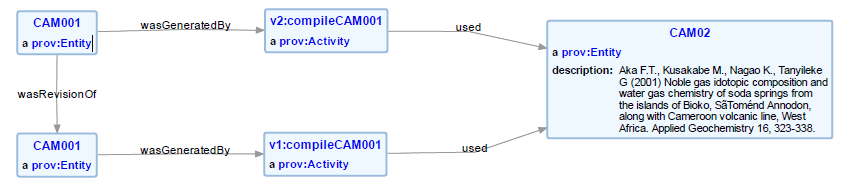
\includegraphics[scale=0.70]{figures/CAM001v1v2.png}
	\caption{Provenance graph for the entry CAM001 entry of the Noble Gas Database.  Other than the labels, the structure of each of the data objects is very much the same.}
	\label{CAM001ProvGraph}
\end{figure}

\section{Versioning Comparison}

The initial challenge for both of these datasets is producing an appropriate mapping between their previous and latest versions.  Through the second compilation process, many columns were removed from the dataset or moved around, and as a result, the identifiers associated with the Attribute in version two did not necessarily correspond to their identifier in version one.  The column headings in the Noble Gas Dataset is stored in the spreadsheet as data and makes it difficult for a general system to automate mapping columns between the two versions since any number of rows may contain metadata information.  Additionally, while the second release of the Noble Gas Dataset did have a document detailing the organization of the columns contained within the dataset, it did not have any information to map entries from the old dataset to the new dataset.  This limits the ability to map and update changes to human actors.  Immediately apparent is that any columns that have a mapping from version one to version two means that these columns (Attributes from the model) will only undergo Modification operations since there exists an associated Attribute in both the previous and current version.  The conclusion then follows that all remaining Attributes (including both columns and rows) belonging to version one were Invalidated and those belonging to version two were Added.  Using this conclusion, we can pre-calculate the Added and Invalidated Attributes and separate any report into changes grouped by operator.

Once a mapping exists between the two versions, a comparison was performed to determine whether an Attribute of the data object changed.  In this case, a simple equality operator was used to determine if anything was modified.  In practice, more advanced or complicated methods can be used to determine equality.  Since, all Additions and Invalidations have already been predetermined, we can output each Modification as we see them.  As is common in versioning, the changes were outputted to a changelog document formatted using HTML.  The idea here is that by providing the changelog in HTML, the changes can be made available online and therefore accessible by data consumers.  Another benefit of providing a changelog in HTML is that the document can be additionally enriched by RDFa.  The changelog document becomes no longer restricted to human consumption, but allows autonomous agents to more intelligently interact with dynamic data systems.  The conceptual model detailed in Chapter~\ref{ch:model} becomes encoded into the changelog and the graph resulting from the log can be extracted automatically.

\begin{figure}
	\centering
	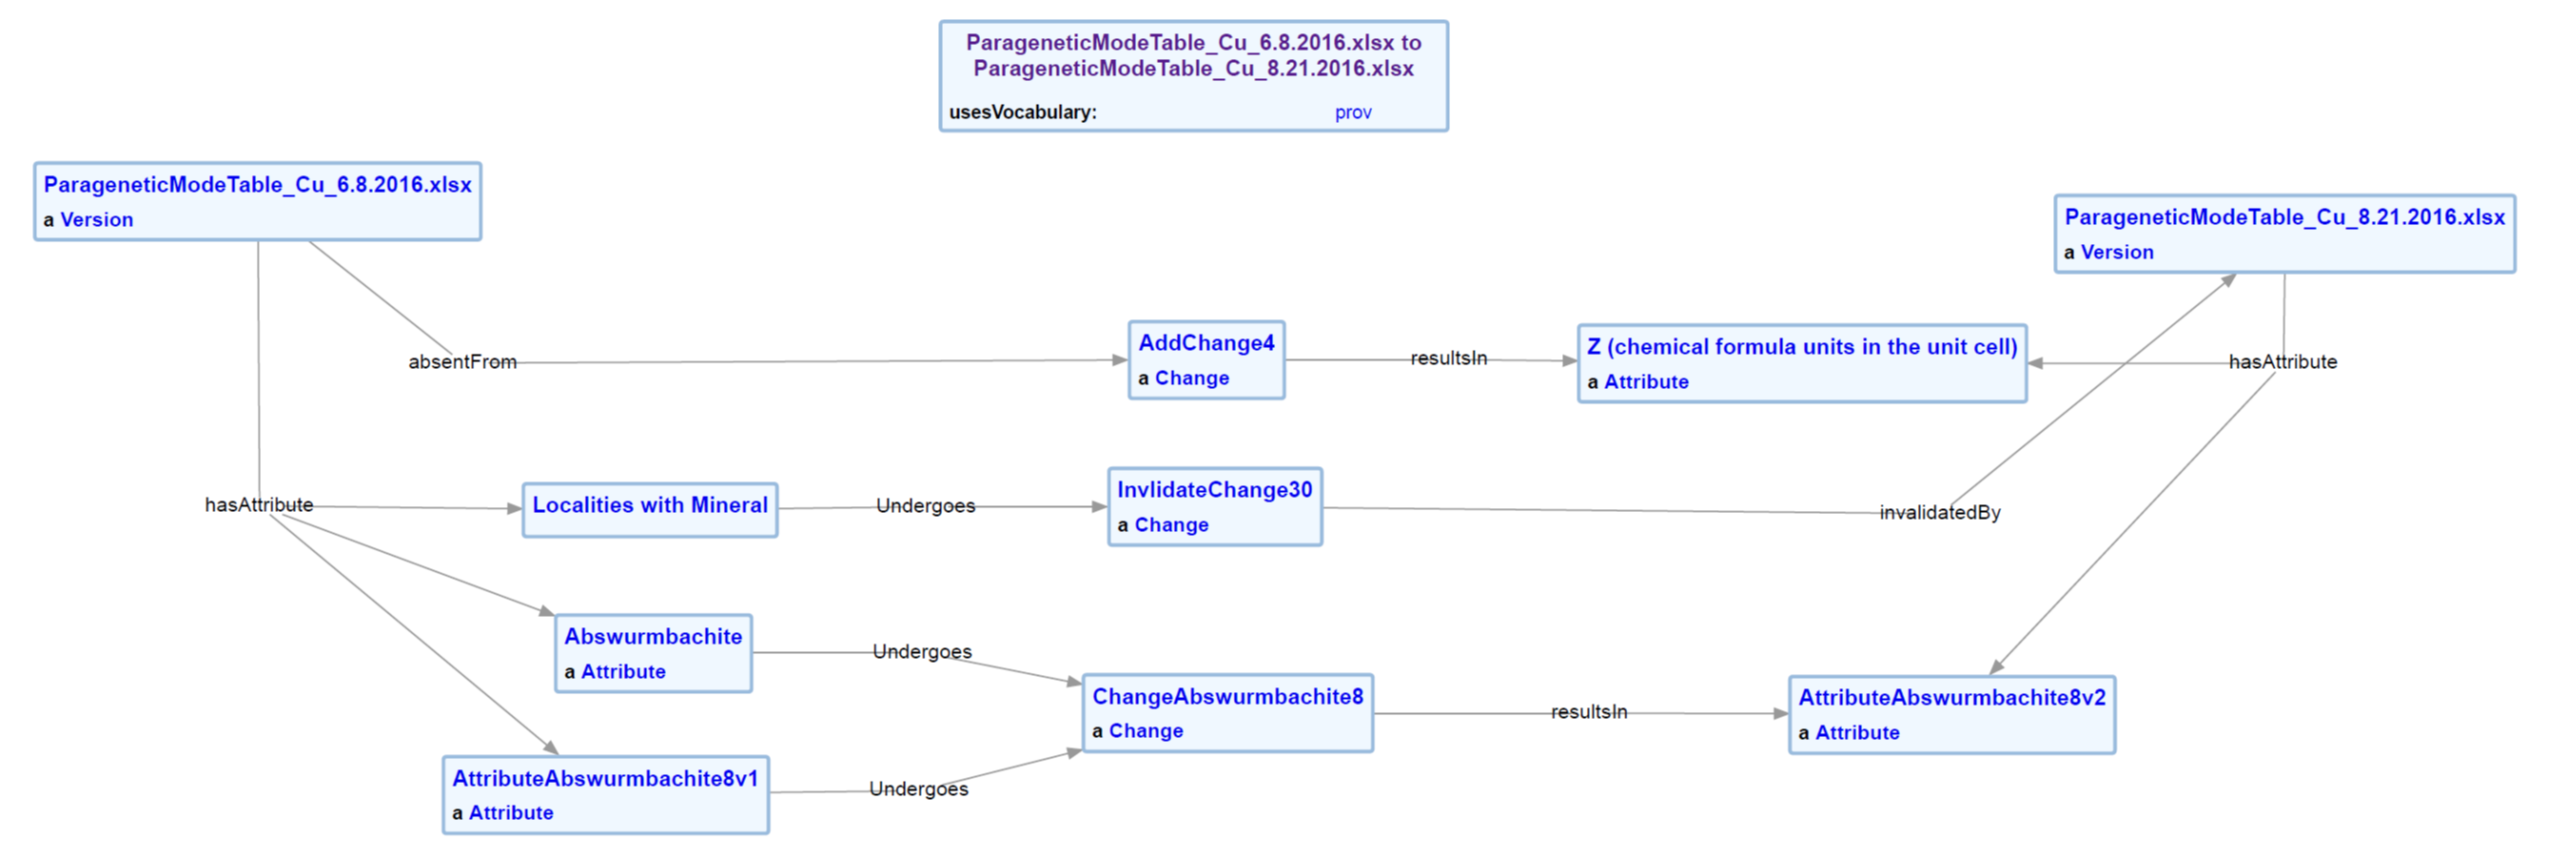
\includegraphics[scale=0.23]{figures/VersioningGraph.png}
	\caption{Versioning Graph representing the linked data graph with selected entries of additions, invalidations, and modifications. }
	\label{CopperGraphVerGraph}
\end{figure}

The resulting graph provides a structure upon which a flow may be calculated.  This becomes an alternative method to determine the provenance distance between two datasets with a much higher fidelity.  As mentioned previously, the Change concept is meant to be sub-classed to provide more freedom to represent the particular change bridging the two versions.  For example, the He Count entry for the Noble Gas Database changed its units from parts per million to cc STP of given gas specie per cc STP of the total gas.  This would be better qualified as a unit change and would be associated with a certain weight in contribution to the total change to the dataset.